\chapter{Verwandte Arbeiten}
\label{kap3}

todo beschreibung

TODO IHME: Dierbei sollte sinnvollerweise auch beschrieben werden, was in der Lösung eigentlich alles enthalten ist. Dabei ging es durchaus auch um Physik, es ging um Visualisierung von Sensorwerten (dazu benötigen Sie noch Informationen von mir) und letztlich auch Planung. Ich denke, dass die Visualisierungaspekte auch für die neue Lösung ein wichtiges Kriterium sind.

todo beschreibung

Dieses Kapitel geht auf die Einzelheiten und die Abläufe der Portierung des Laufplaners in das \acf{ROS} und Gazebo ein. Zunächst werden die wesentlichen Aspekte des bestehenden Laufplaners analysiert und mögliche Herausforderungen dargestellt. Dann wird ein eigenes \ac{ROS}-Paket entworfen, welches die Basis für den neuen Laufplaner darstellt. Das Kapitel stellt alle nötigen Schritte dar, um die Simulation aufzusetzen und den Laufplanungsalgorithmus zu migrieren.

\section{Analyse bestehender Laufplaner}

Der von André Herms \autocite{herms2004} und von Uli Ruffler \autocite{ruffler2006} weiterentwickelte Laufplaner für den \emph{Lauron} basiert auf der 3D-Bibliothek OpenInventor \autocite{inventor}. Dieses Toolkit basiert wiederum auf OpenGL und ist in C++ implementiert. Des Weiteren ist es objektorientiert und daher orientiert sich auch der Laufplaner an diesem Programmierstil. Auf Grund dieser Tatsache existieren Klassen bzw. Objekte, die nun beschrieben werden:
\begin{itemize}
  \item \emph{World}: speichert die Objekte der Sicht auf die Landschaft und den Roboter. 
  \item \emph{Terrain}: enthält die Informationen über die Höhenkarte.
  \item \emph{Eyes}: stellt die Sicht auf die Landschaft dar.
  \item \emph{Robot}: ist verantwortlich für die Robotersteuerung und definiert außerdem die inneren Objekte \emph{Head} und \emph{Leg}.
  
\begin{figure}[t!]
  \centering
  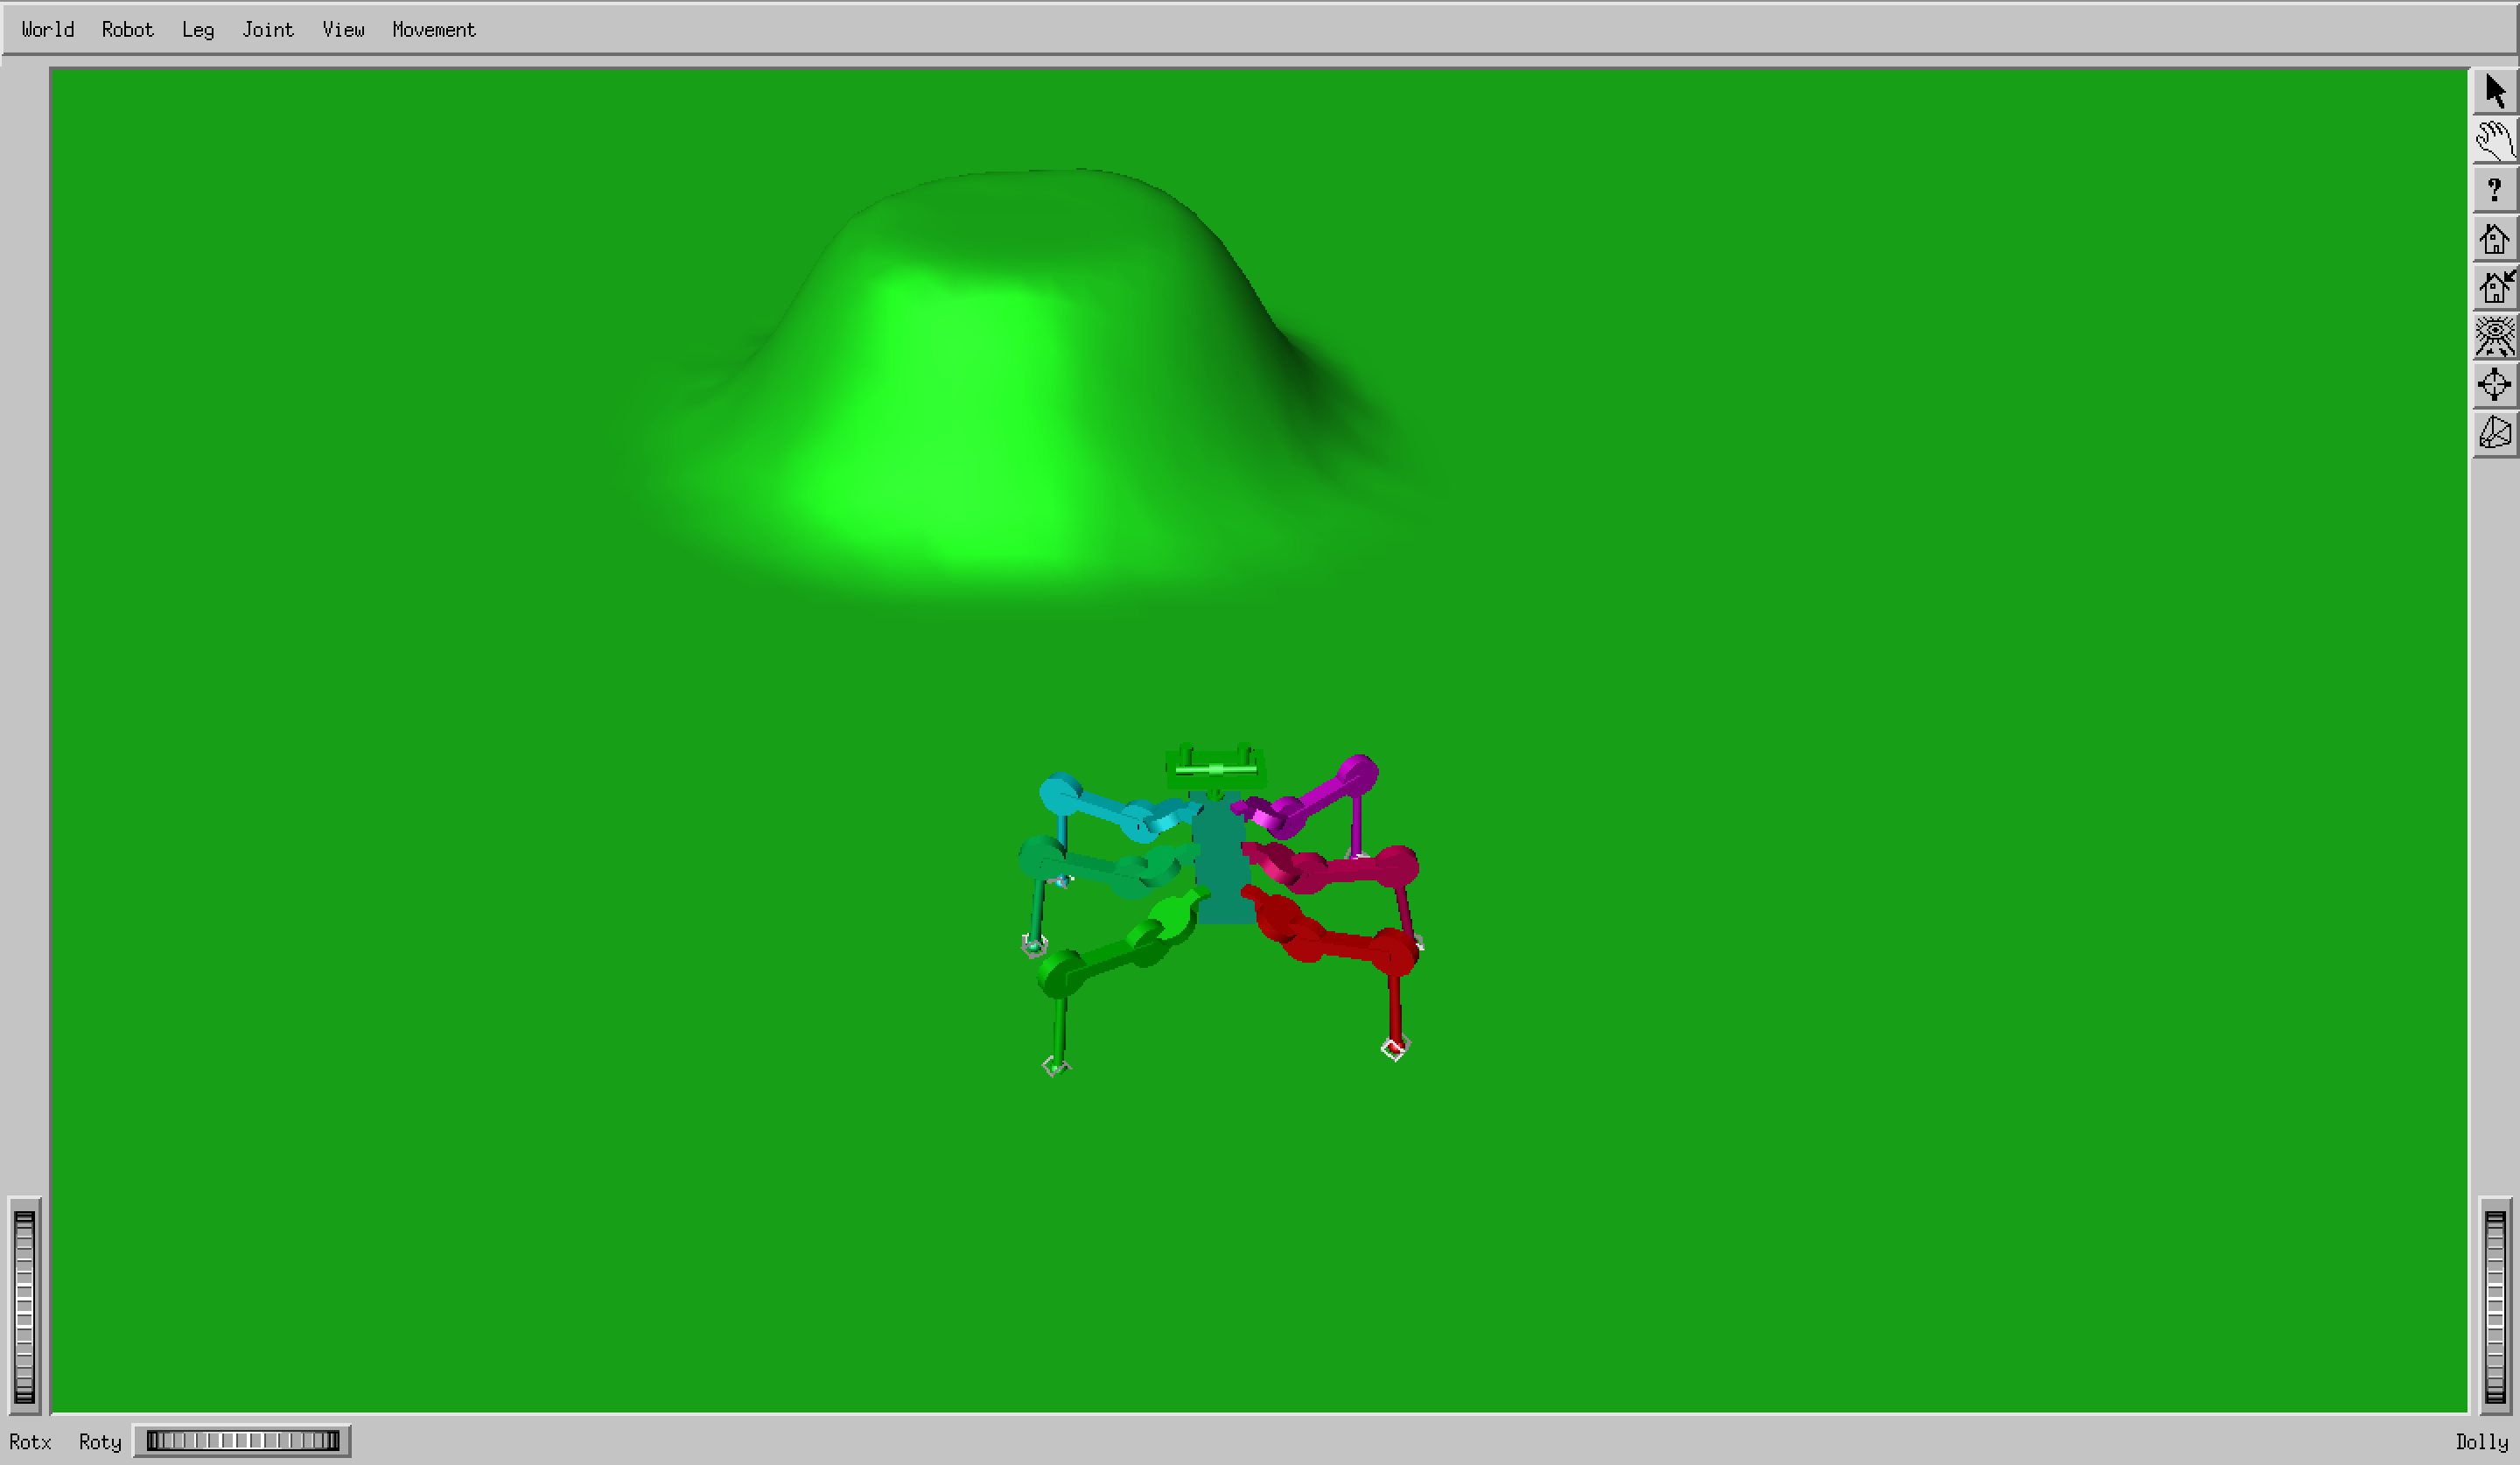
\includegraphics[height=8cm]{kapitel4/openinventor-lauron}
  \caption{Screenshot aus der OpenInventor-Umgebung}
  \label{Kap4:OpenInventorLauron}
\end{figure}

Für jedes dieser Darstellungsobjekt in OpenInventor wird ein \emph{SoSeperator} benötigt. Da der Name dieses Objekts einzigartig sein muss, sind die Objekte auch nur einmalig nutzbar. Dies erschwert die Aufgabe, später einmal mehrere Roboter gleichzeitig in der Simulation zu testen. Code-technisch sollte das dem Design-Pattern \emph{Singleton} folgen. Der Laufplaner sichert diese allerdings nicht derart ab.

Des Weiteren stellt das Terrain-Objekt die Höhenkarte der Landschaft in OpenInventor zur Verfügung. Dies entspricht nicht dem, was dem Roboter tatsächlich an Kartenmaterial zur Verfügung hat. Diese Tatsache erschwert die Portierung auf ein anderes System, da eine Möglichkeit geschaffen werden muss, dem Roboter beizubringen, was er sieht, um weiterhin mit Höhenangaben arbeiten zu können.

Eine Konfigurationsdatei existiert bereits in dieser Umgebung, die es ermöglichen soll, auch andere Robotermodelle zu testen. Genau dieser Fall ist an dieser Stelle interessant, da die Portierung des Laufplaners auf den \amph{Akrobat} geschehen soll. Diese wird für den Laufalgorithmus allerdings nicht genutzt, da dort Roboterangaben direkt im Quelltext definiert sind.

Weiterhin wird die aktuelle Fußkonfiguration sowie die Fußposition getrennt voneinander gespeichert. Die Fußkonfiguration ist in einer Bitlogik gespeichert. Dies ist sehr nützlich um Speicherplatz zu sparen, macht auf der anderen Seite das Finden von Fehlern allerdings schwieriger.